\section{Case Study}

In this section, we apply the method described above to study the case of Shenzhen. We introduce the several cases to demonstrate the usage and effectiveness of the system.

%The cases of analysis how individuals use the city are derived to demonstrate the powers. We believe this work would be one of the natural steps into research of social understanding of the city.

\subsection{Case 1: Work-life Balance VS Income/Education}


% \begin{figure}
% \centering
% \subfigure[Top aristocracy.]{
% \resizebox*{4.4cm}{!}{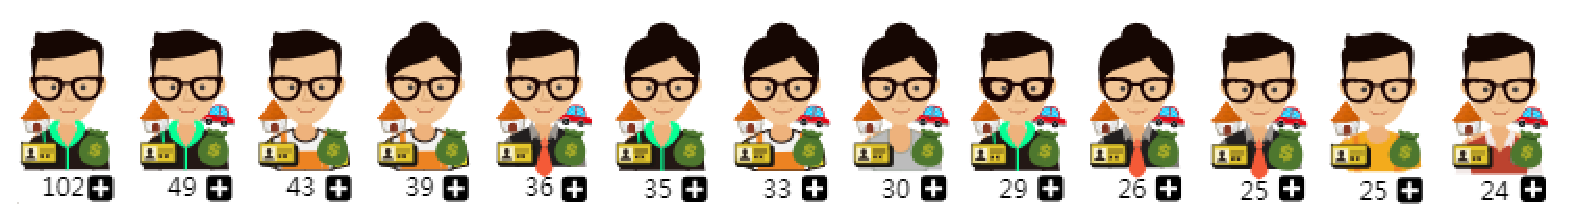
\includegraphics{pictures/case111.eps}}}\hspace{5pt}
% \subfigure[The underclass.]{
% \resizebox*{4.4cm}{!}{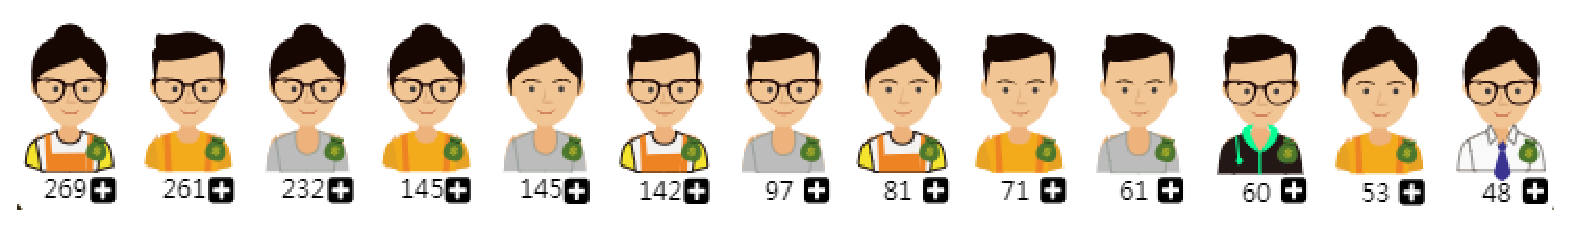
\includegraphics{pictures/case112.eps}}}\hspace{5pt}
% \subfigure[New rich.]{
% \resizebox*{4.4cm}{!}{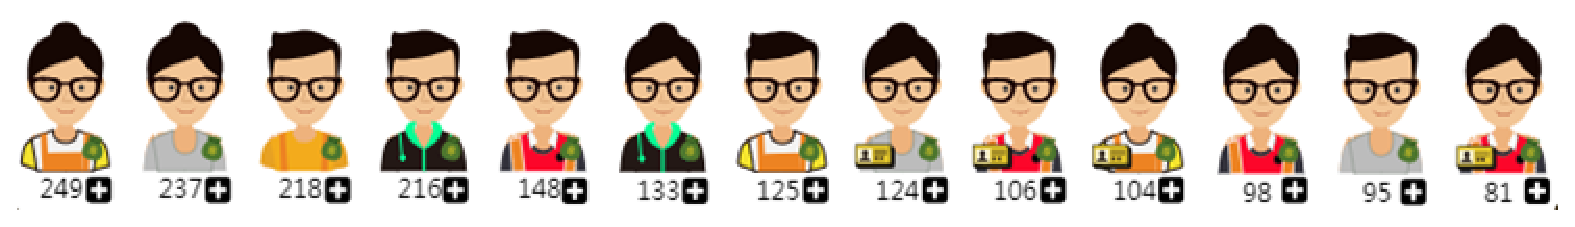
\includegraphics{pictures/case113.eps}}}\hspace{5pt}
% \subfigure[Antizen.]{
% \resizebox*{4.4cm}{!}{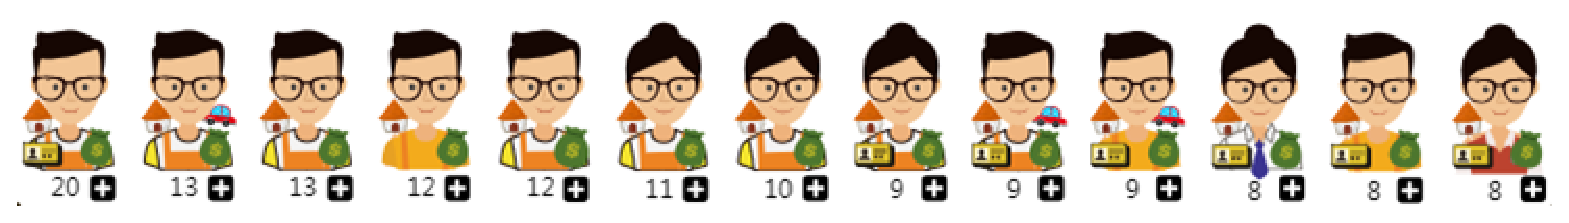
\includegraphics{pictures/case114.eps}}}\hspace{5pt}
% \caption{XXXXXX of different groups.}
% \label{case11}
% \end{figure}


% \begin{figure}
% \centering
% \subfigure[Top aristocracy.]{
% \resizebox*{4.4cm}{!}{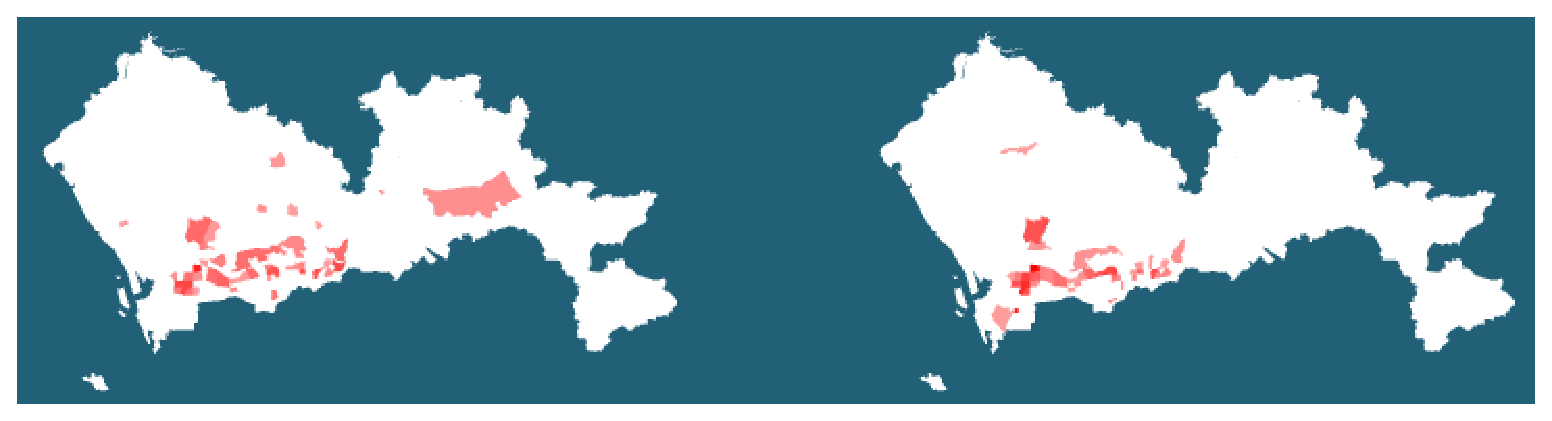
\includegraphics{pictures/case121.eps}}}\hspace{5pt}
% \subfigure[The underclass.]{
% \resizebox*{4.4cm}{!}{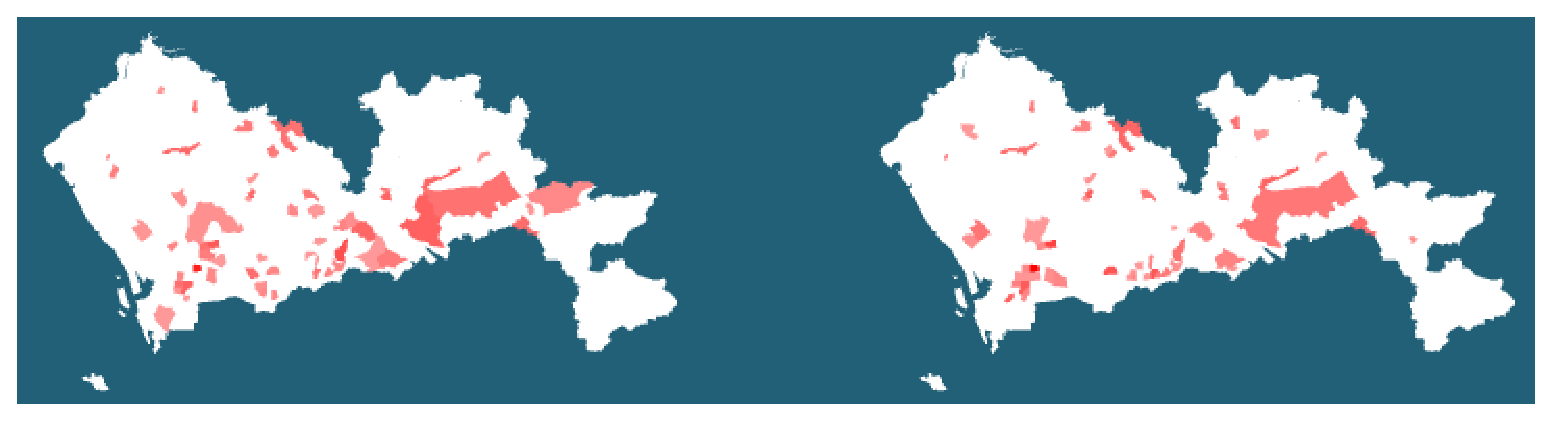
\includegraphics{pictures/case122.eps}}}\hspace{5pt}
% \subfigure[New rich.]{
% \resizebox*{4.4cm}{!}{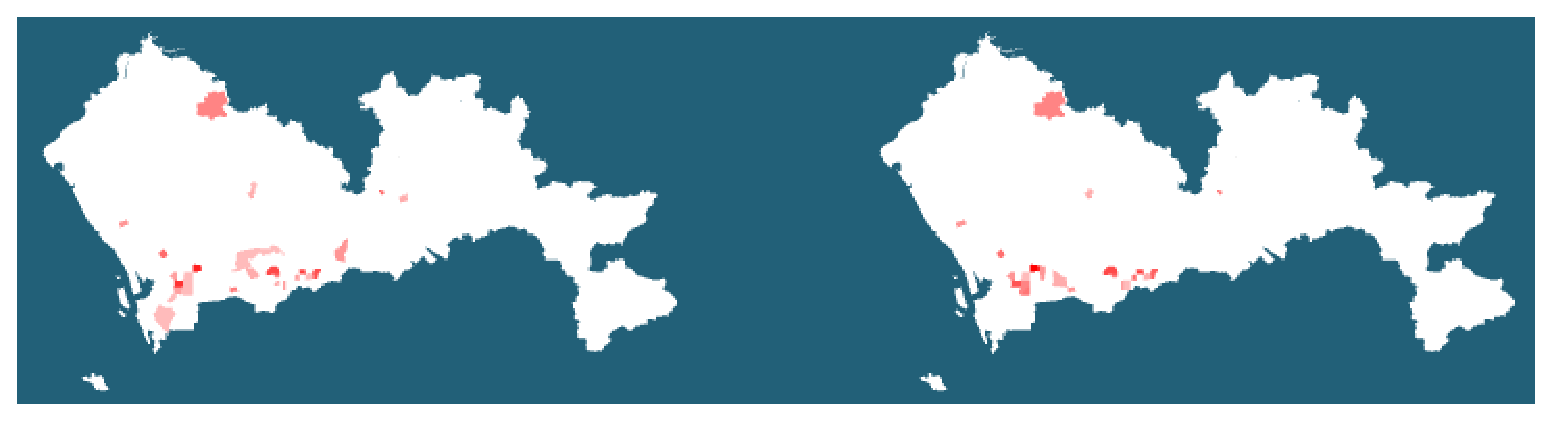
\includegraphics{pictures/case123.eps}}}\hspace{5pt}
% \subfigure[Antizen.]{
% \resizebox*{4.4cm}{!}{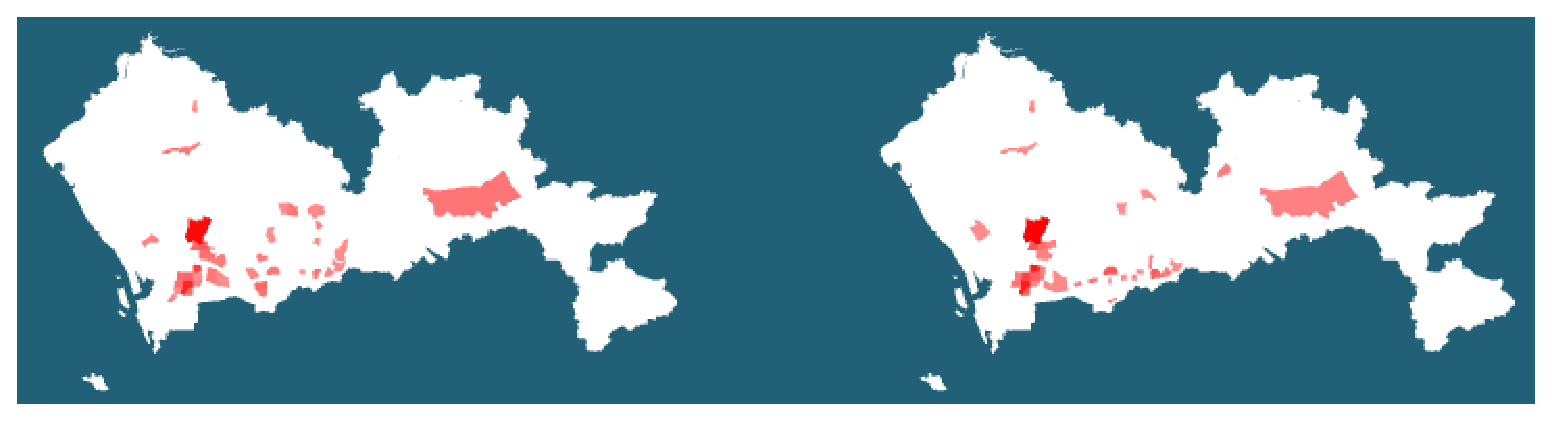
\includegraphics{pictures/case124.eps}}}\hspace{5pt}
% \caption{}
% \label{case12}
% \end{figure}


This work is inspired and motivated by the implication in science fiction~\textit{Folding Beijing}, which is that people are categorized into three classes and behave in the parallel spatial-temporal patterns. The first cast explores whether the folding city exists in reality or not.

\begin{figure}[htb!]
 \centering % avoid the use of \begin{center}...\end{center} and use \centering instead (more compact)
 \includegraphics[width=\columnwidth]{pictures/case1_1}
 \caption{Four Groups Divided by Income and Education Characteristics}
 \label{case11}
\end{figure}

Although it is incomplete, income and education are two of the most essential characteristics to tag an individual with a good resource or not. 
As Figure~\ref{case11} shows, taking income and education as the two dimensions, taking 300K yuan as the border between high and low income and an undergraduate bachelor degree as the border between high and low education level, four different groups are generated in the four quadrants. In the first quadrant, individuals are rich and well educated, who are in a group of so-called \textit{top aristocracy}. The second quadrant holds the group of \textit{new rich}, i.e., individuals with high income but low education income. In the third quadrant, they are the \textit{underclass} who has both low income and education level. The fourth quadrant is \textit{Antizen}, which is a new word to describe people have a good education but earn little. 


Figure~\ref{case11} shows the top 12 profiles with the maximum population in each group. In each group, other characteristics surprisingly demonstrate the high correlation to income and education. For example, almost all of the \textit{top aristocracy} is with the residential license,  house, and car. On the contrary, \textit{underclass} do not have the residential license residence, neither the house nor the car. Most of \textit{New rich} has a house and work in the service industry.  

Before diving into the complex mobility pattern analysis, we explore the home distribution of the four groups. As Figure~\ref{case12} shows, \textit{top aristocracy} and most of \textit{new rich} live concentrated in the downtown area of Shenzhen, where the living cost is higher, especially the housing cost. A small part of \textit{new rich} lives far away from the downtown, maybe because they don't have to work in downtown. The \textit{underclass} distribute more dispersively all over the whole city. Compared to the rich, they prefer the outer space because of the lower living cost. Lots of \textit{antizen} live in Nanshan District, where there are many universities and high-tech industrial parks full of well educated people. 

\begin{figure}[htb!]
 \centering % avoid the use of \begin{center}...\end{center} and use \centering instead (more compact)
 \includegraphics[width=\columnwidth]{pictures/case1_2}
 \caption{Home Distributions of the Four Groups}
 \label{case12}
\end{figure}


% To understand how citizens live in the city, there are two crucial aspects to be known: during the night where they sleep, and where do they do during the daytime. ``Home location" could answer the first question. The second one is harder to summarise because of the complexity of daytime activities. In our method, we divide daytime mobility activities into 

To have a better knowledge of mobility patterns of the four groups, trips are categorized into three categories, ``home", ``work'' for regular trips with the purpose of going home, work (or school for students), ``other'' for irregular trips with the purpose of shopping, visiting friends. Figure~\ref{case13}(a) shows the 2.5D overview of the three kinds of traveling categories. Each TAZ is grown to the same height, i.e., the unit one, and the height proportion of each traveling categories encodes the percentage of certain purpose in the whole, pink for ``others'', blue for ``work'' and green for ``home''. Although inside TAZ prisms are blocked in the Figure~\ref{case13}, our attention is drawn to the lifestyle of \textit{New Rich}. It is founded that the \textit{New Rich} travel for ``other'' purpose a lot, compared to other groups. To explore further, the detail slicing (introduced in Section~\ref{subsec:25D}) is applied to the four groups. Figure~\ref{case13}(b) shows three slices. It can be seen that individuals with low income (\textit{underclass} and \textit{antizen}) spend relatively more time on work, especially the \textit{underclass}. Working percentage is very small in-group \textit{new rich}. They live a more diverse lifestyle because they do many other things (the pink ones) except working.


\begin{figure}[htb!]
 \centering % avoid the use of \begin{center}...\end{center} and use \centering instead (more compact)
 \includegraphics[width=\columnwidth]{pictures/case1_3}
 \caption{Mobility Patterns of ``work", ``home" and ``not essential" of the Four Groups: (a) the overview of the three pecentage; (b) three slices for detailed comparison.}
 \label{case13}
\end{figure}

% By comparing them, it can be seen that the poor spend more time on work, especially ``the underclass". Working percentage is really small in-group ``new rich". They have diverse lives because they do many other things except for working.


% \begin{figure}
%   \centering
%   \includegraphics[width=0.95\linewidth]{pictures/case1_4}
%   \caption{Examples of XXXXX.}
%   \label{case14}
% \end{figure}
% two categories to capture mobility patterns. ``routine activity" is made up with ``go to work", ``go to school" and ``go back home". Movements with other purposes are ``not essential". People do these movement activities due to their personal willingness and living style. Therefore, ``home location", ``working location" and ``not essential" activity space outline one's living space. Our system meets this requirement.

% In Fig. \ref{case13}, the distributions of ``essential" activity including ``go to work" and ``go home", and ``not essential activity" are shown. 

% From the dimension of space, ``new rich" prefer to live in the west of the city. They do not go south-east in most times. Other three groups reach the whole city. The height of the bar stands for the percentage of each kind of activity. Higher height means that the group has more willingness and cost more time in ``, not the essential activity", while lower height means more time on work. As we described in Section XXX, �ڵ�����, ����ʹ���������� Fig. \ref{case14} give three examples within each group to check the detailed information in the 2.5D graph. By comparing them, it can be seen that the poor spend more time on work, especially ``the underclass". Working percentage is really small in-group ``new rich". They have diverse lives because they do many other things except for working.


\subsection{Case 2: Home-work Distance VS Income/House}


\begin{figure}[htb!]
 \centering % avoid the use of \begin{center}...\end{center} and use \centering instead (more compact)
 \includegraphics[width=\columnwidth]{pictures/case2}
 \caption{Home-work distances of different groups: (a) with different salary levels; (b) with or without house.}
 \label{case2}
\end{figure}

% \begin{figure}
% \centering
% \subfigure[Group of people whose income more than 500,000yuan per year.]{
% \resizebox*{4.4cm}{!}{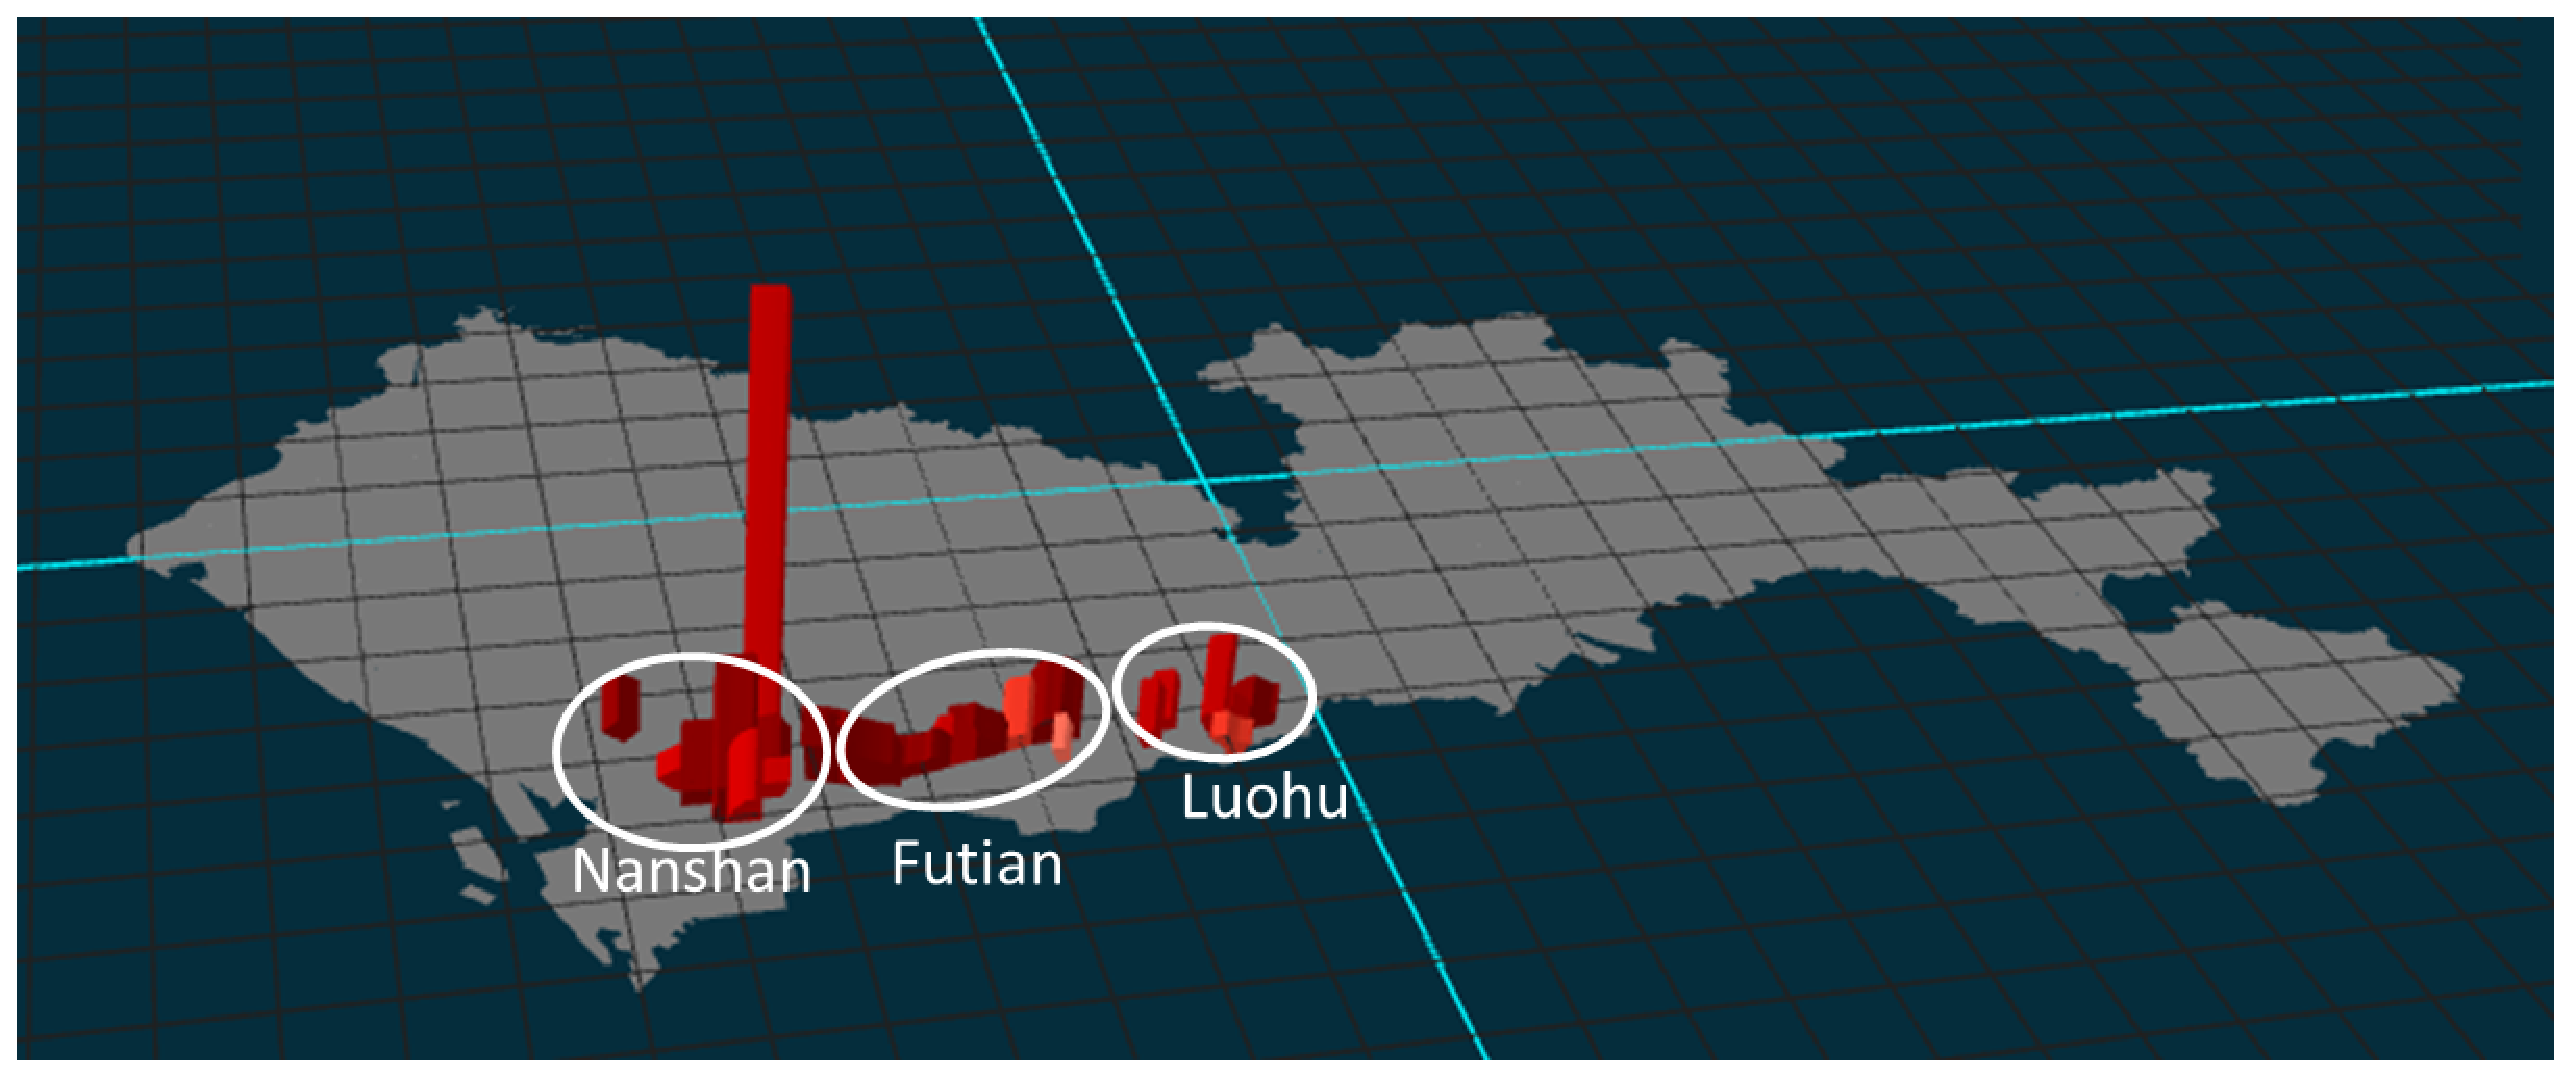
\includegraphics{pictures/case21.eps}}}\hspace{5pt}
% \subfigure[Group of people whose income between 200,000 yuan to 300,000 yuan per year.]{
% \resizebox*{4.4cm}{!}{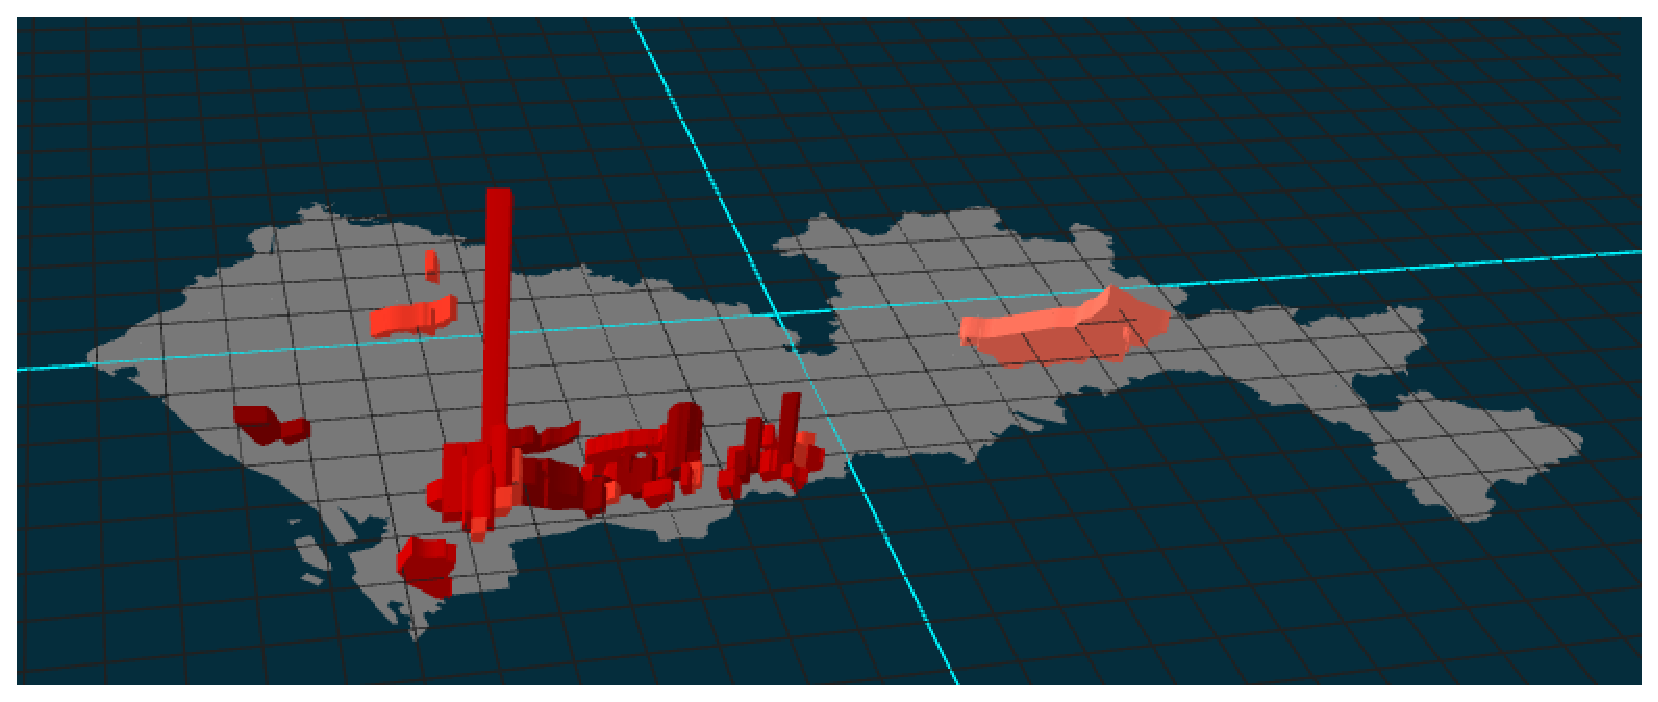
\includegraphics{pictures/case22.eps}}}\hspace{5pt}
% \subfigure[Group of people whose income less than 100,000yuan per year.]{
% \resizebox*{4.4cm}{!}{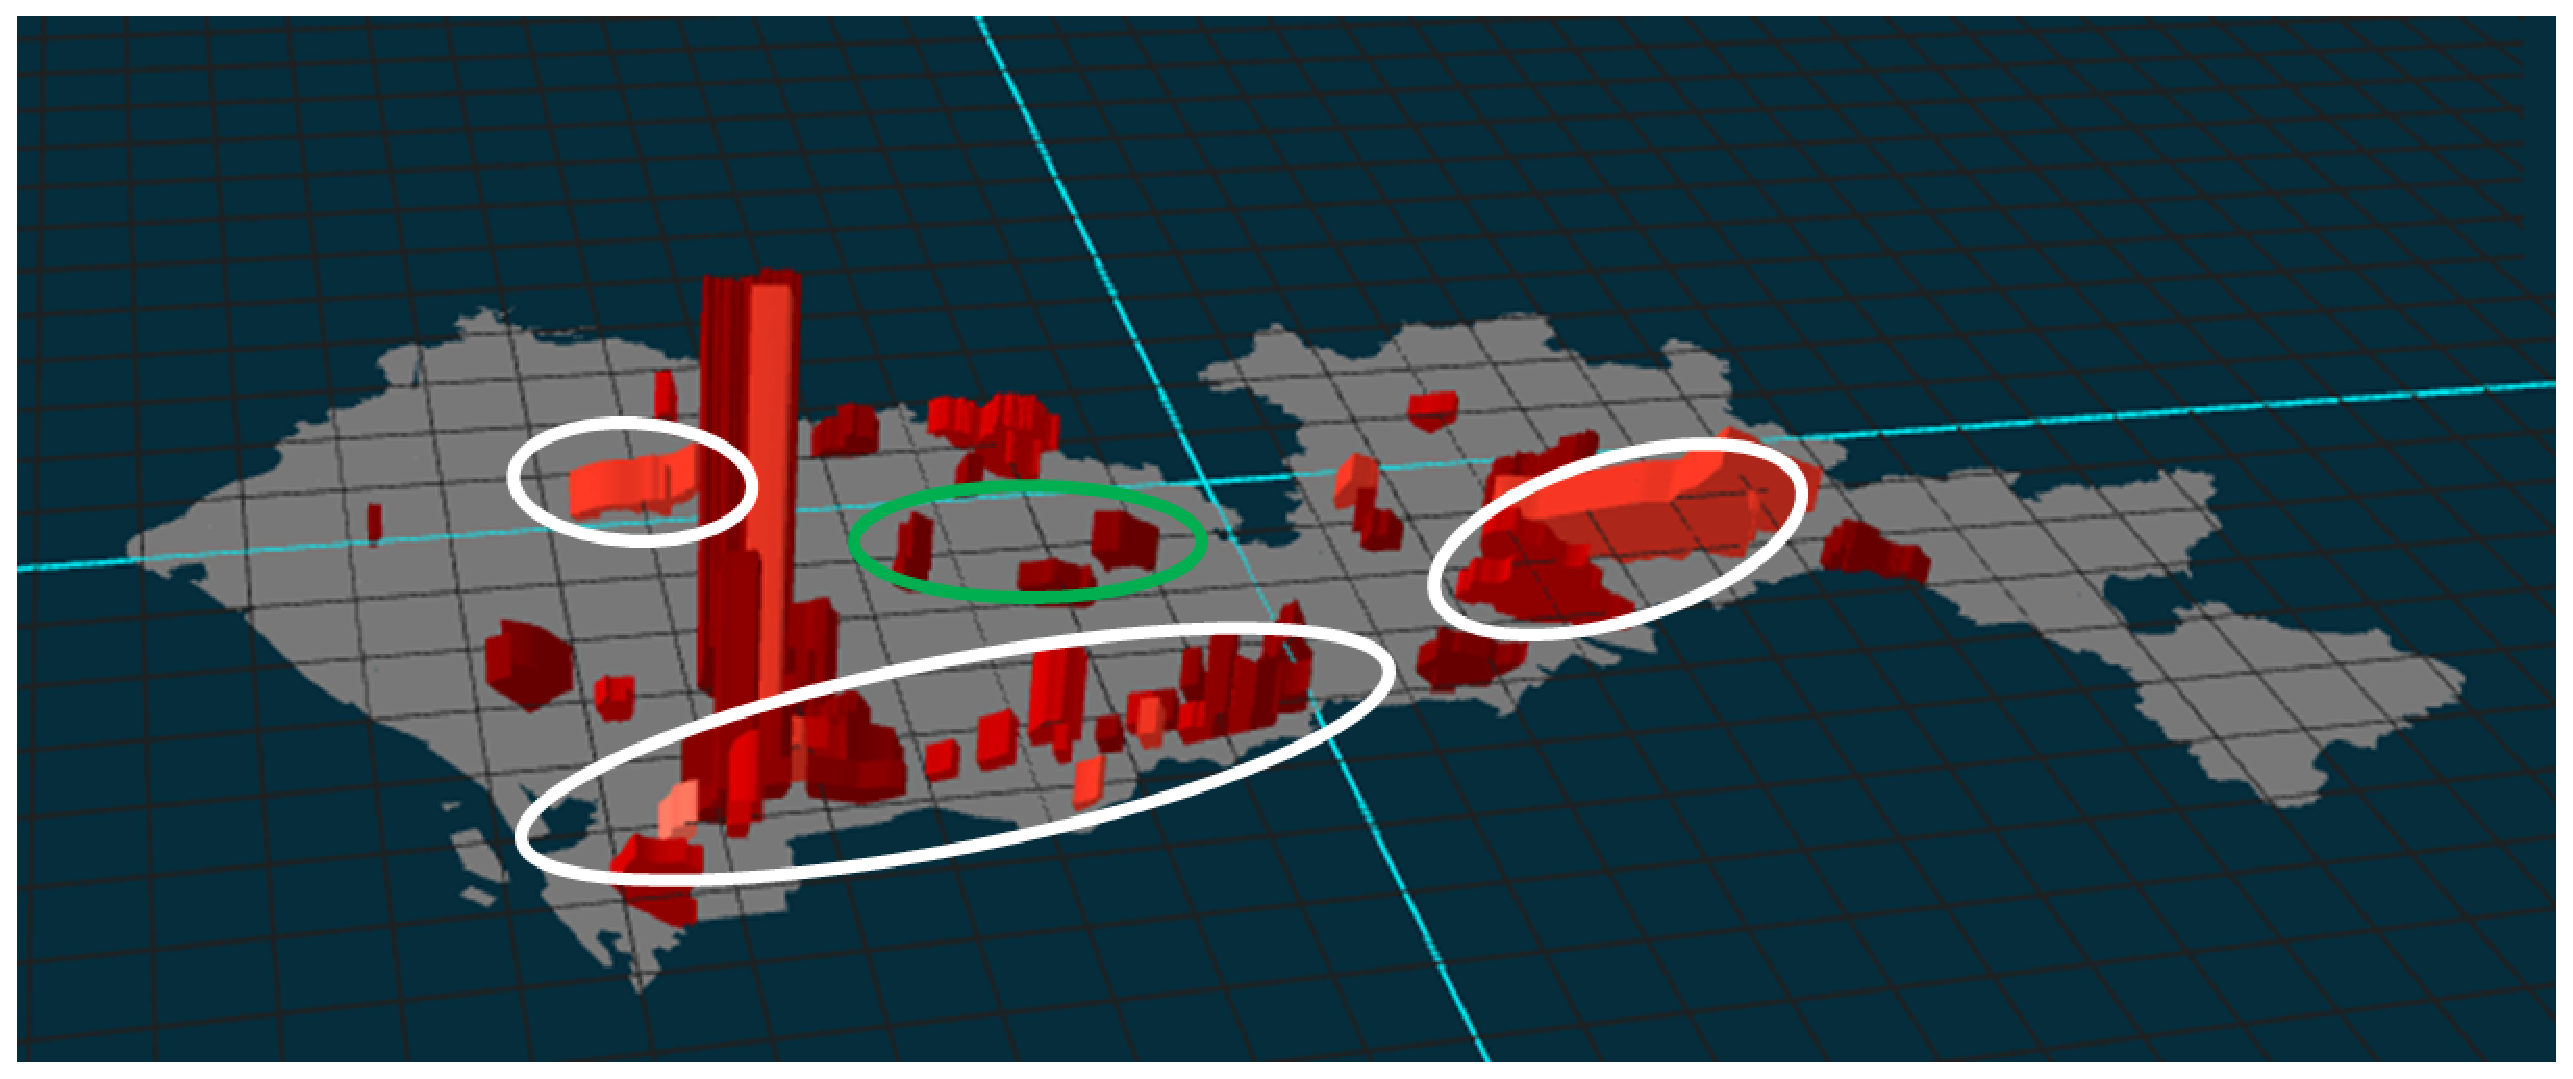
\includegraphics{pictures/case23.eps}}}\hspace{5pt}
% \subfigure[Group of people who owe house.]{
% \resizebox*{4.4cm}{!}{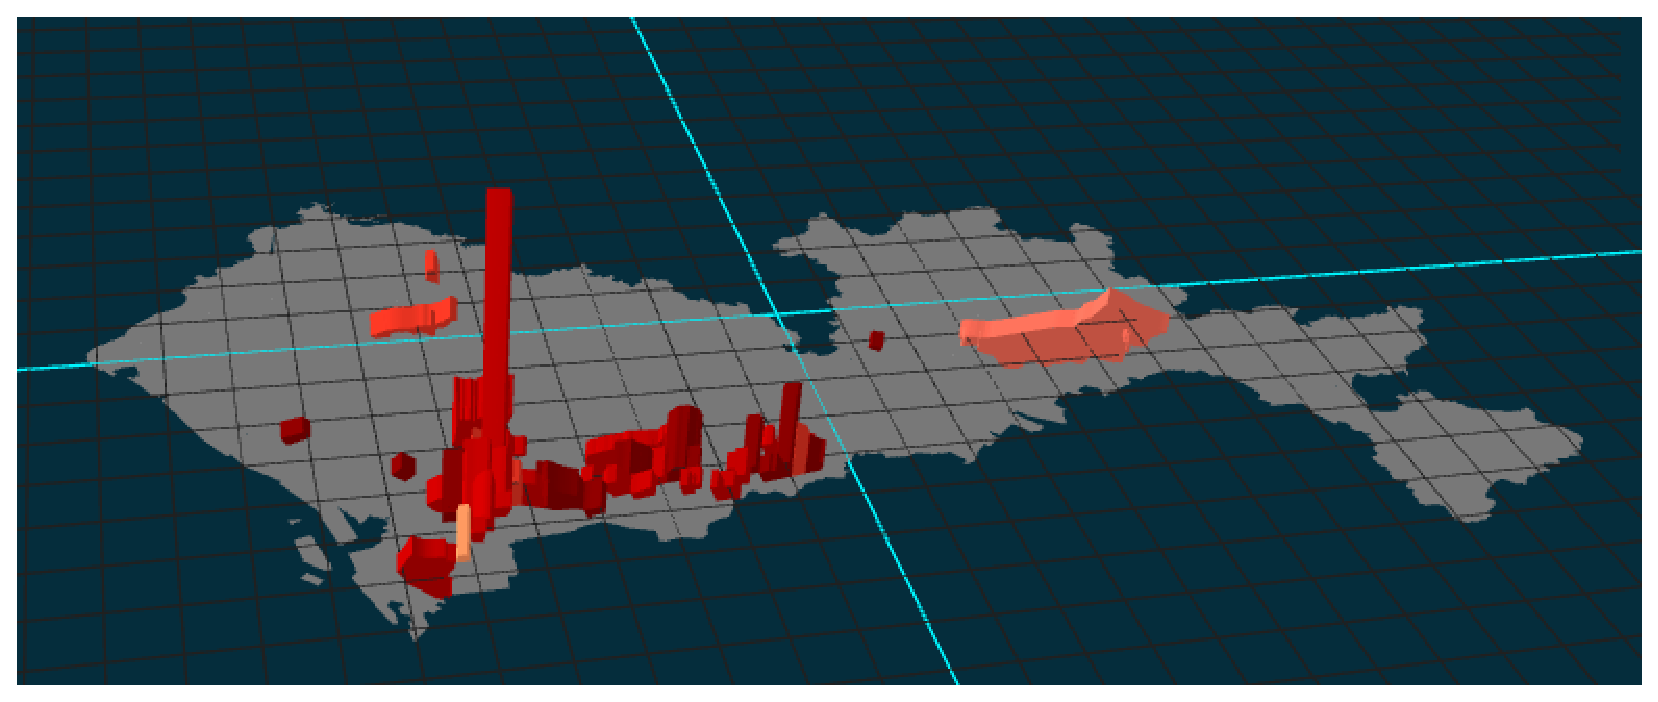
\includegraphics{pictures/case24.eps}}}\hspace{5pt}
% \subfigure[Group of people who rent house.]{
% \resizebox*{4.4cm}{!}{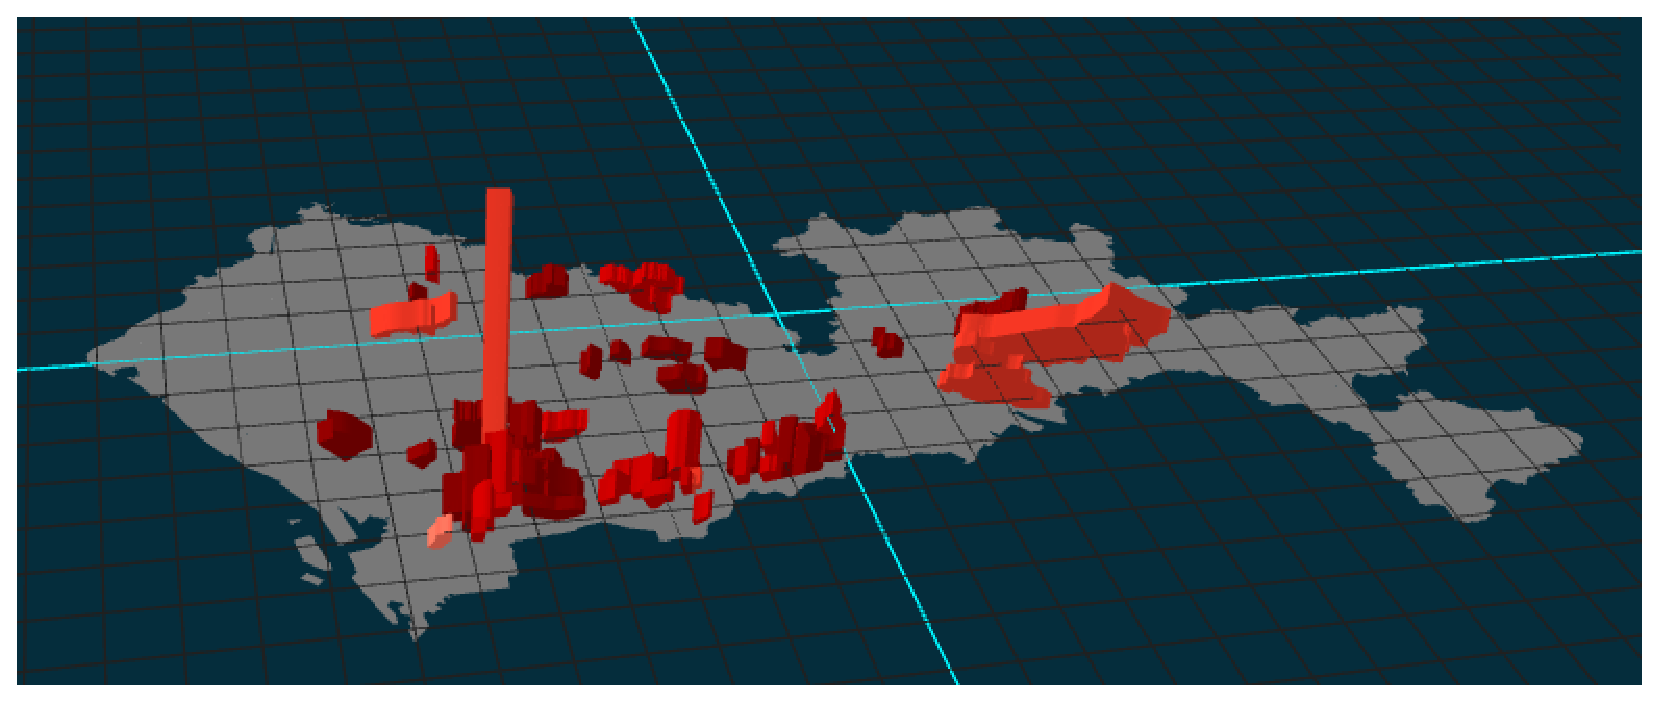
\includegraphics{pictures/case25.eps}}}\hspace{5pt}
% \caption{Home-work distances of different groups.}
% \label{case2}
% \end{figure}

Home-work distance is an essential metric in economics, geography, and sociology. It refers to the distance between house and workplace. It is influenced by many factors like transportation, housing, land use, etc. Understanding the home-work distance of a region helps to evaluate whether the region is well planned or not. In this case, we demonstrate our system's help in home-work distance understanding.

Considering income potentially determines where people live, we use income as the characteristics to select three groups, the group over 500K, the group during 200-300K and the group less than 100K. In Figure~\ref{case2}, the height of the bar stands for visiting frequency of the TAZ and its color encodes the average home-work distance, red for close and yellow for far. As Figure~\ref{case2}(a) shows, for all the three groups in different income levels, most of the TAZs have dark red or red color which indicates the home-work distance is generally short, especially in downtown. Only those with less than 100K salary work outside the center, such as the space in the green circle. When comparing the three groups in the downtown area, it is seen that it takes more time to go to work in Futian District as the decrease of the income. 

We explore the home-work distance of groups with and without a house. 
Figure~\ref{case2}(b) shows the close-up views. It is found that the Nanshan District has a shorter home-work distance for individuals without a house, while Futian District has shorter for those with a house. Nanshan is relatively newer to Futian so that there might be more easily-accessible houses to be rent.

  % District belongs to all but Futian District belongs to the rich. The poor could rent house living in Nanshan and Luohu to enjoy short home-work distance. In Futian, only the rich working there have short home-work distance. There may be no much housing for rent.

 % From the figure, it is seen that the working locations are mainly in three areas which are circled in white in Fig. \ref{case2}(c). Space in green circle is another hot working area which only is preferred by the poor.
% On the whole, home-work distance is short in Shenzhen for most of the TAZs with different groups have a darker color, especially in downtown. When focusing on the downtown area, it is seen that there are differences between Futian District with the other two. By comparing three groups distinguished by income, it takes more time to work in Futian District with the decrease of the income. Meanwhile, the opposite is true in others. In combination with Fig. \ref{case2}(d) and Fig. \ref{case2}(e), 


\subsection{Case 3: Life-style VS Jobs}

% \begin{figure}
% \centering
% \subfigure[Officer.]{
% \resizebox*{4.4cm}{!}{\includegraphics{pictures/311.eps}}}\hspace{5pt}
% \subfigure[Workman.]{
% \resizebox*{4.4cm}{!}{\includegraphics{pictures/321.eps}}}\hspace{5pt}
% \subfigure[Student.]{
% \resizebox*{4.4cm}{!}{\includegraphics{pictures/331.eps}}}\hspace{5pt}
% \subfigure[Businessman.]{
% \resizebox*{4.4cm}{!}{\includegraphics{pictures/341.eps}}}\hspace{5pt}
% \caption{Percentage of movement with purposes in group of different jobs.}
% \label{case31}
% \end{figure}

In this case, we explore the correlation between mobility patterns with the job, to see whether the job has an impact on the movement. Officer, workman, student, and businessman are selected as examples and the population of trips for certain purposes is shown In Figure~\ref{case3}. The height of bars encodes the amount of visit to each TAZ, and color encodes the traveling purpose. There are 10 different kinds of traveling purposes. For quick linking between color and purposes, the regular trips such as go to work, school and home are dyed in cold color, and the irregular trips such as go shopping, hospital, etc, are dyed in the warm color. As Figure~\ref{case3} shows, for officers, the TAZs changes dramatically in height. Some TAZs have much more visiting than others because officers are more constrained to work in some buildings than individuals with other jobs. The relative percentage of irregular activity differs for the four groups. For Workman, about 80 percent of movements are the regular purpose, either go to work or go back home. For students, the percentage becomes to be about 50 percentage. Compared to them, officer and businessman have more flexible and diversified lifestyle.




% Each social attribute has an impact on movement patterns. There are 9 kinds of jobs in the data which offers rich information. Therefore, in this case, we use ``job" as the target social attribute to explore its influence on citizens' movement patterns.

% At first, with 2.5D spatial visual form, we learn what people move for and the percentage of movements with a given purpose. 

% The height of each bar stands for the number of movements to the TAZ. Purposes are encoded in color as the legends show. From the perspective of the height of bars, it is seen that the amount of visitors to each TAZ of officers is really different. Several TAZs have the dominant visiting. In Figure~\ref{case3}(a), the heights of yellow bars and rose red bars in different TAZs have great differed. This phenomenon is not that obvious in other three groups. In addition, the percentage of ``not essential" activity differs. For Workman, about 80 percent of movements are ``essential" ones. For students, the percentage becomes to be about 50 percentage. Compared to them, officer and businessman have more flexible and diversified lives.


\begin{figure}[htb!]
 \centering % avoid the use of \begin{center}...\end{center} and use \centering instead (more compact)
 \includegraphics[width=\columnwidth]{pictures/case3}
 \caption{Trip purposes distribution of four groups with different jobs}
 \label{case3}
\end{figure}

Next, we concentrated on one purpose to see whether it is related to jobs. Here we use ``dinner or entertainment" as the example. As Fig \ref{case32} shows, the height of TAZ bars represents the visiting amount of trips for dinner or entertainment. Color stands for moving distance to reach this TAZ. As we can see, officers prefer to entertain in the downtown area, while workmen cover a larger area. Students tend to concentrate on Nanshan district, probably near schools. For the businessmen, they go lots of places for dinner or entertainment. The biggest difference with other groups is that they would travel a long distance to go somewhere far from downtown areas. 

\begin{figure}[htb!]
 \centering % avoid the use of \begin{center}...\end{center} and use \centering instead (more compact)
 \includegraphics[width=\columnwidth]{pictures/case3_2}
 \caption{The ``dinner or entertain" purpose of four groups with different jobs}
 \label{case32}
\end{figure}

% \begin{figure}
% \centering
% \subfigure[Officer.]{
% \resizebox*{4.4cm}{!}{\includegraphics{pictures/314.eps}}}\hspace{5pt}
% \subfigure[Workman.]{
% \resizebox*{4.4cm}{!}{\includegraphics{pictures/324.eps}}}\hspace{5pt}
% \subfigure[Student.]{
% \resizebox*{4.4cm}{!}{\includegraphics{pictures/334.eps}}}\hspace{5pt}
% \subfigure[Businessman.]{
% \resizebox*{4.4cm}{!}{\includegraphics{pictures/344.eps}}}\hspace{5pt}
% \caption{}
% \label{case32}
% \end{figure}

